
\thispagestyle{plain}

\chapter{Konfiguration der Anwendung}\label{c_config}
Die Konfiguration der Anwendung findet hauptsächlich über die \emph{application.properties} Datei statt. Hier können sämtliche Werte wie zum Beispiel Datenbank-URL, Logging-Einstellung usw. festgelegt werden. Die Konfigurationsdateien befinden sich im Verzeichnis \emph{resources}. Siehe Listing \ref{lst:appprops} als Beispiel.

   \begin{lstlisting}[caption={application.properties},label={lst:appprops},language=Java]
app.name=weFactor

# IDENTITY (ContextIdApplicationContextInitializer)
spring.application.name=weFactor

logging.level.org.springframework.web: DEBUG
logging.level.org.hibernate: ERROR

# THYMELEAF (ThymeleafAutoConfiguration)
spring.thymeleaf.encoding=UTF-8
spring.thymeleaf.content-type=text/html


# EMBEDDED SERVER CONFIGURATION (ServerProperties)
server.tomcat.uri-encoding = UTF-8

spring.mvc.locale=en_UK
spring.mvc.date-format= dd/MM/yyyy

# INTERNATIONALIZATION (MessageSourceAutoConfiguration)
spring.messages.basename=messages
spring.messages.cacheSeconds=-1
spring.messages.encoding=UTF-8

    
   \end{lstlisting}
   Eine ausführliche Liste der Einstellmöglichkeiten ist in der Spring Dokumentation\footnote{\url{http://docs.spring.io/spring-boot/docs/current/reference/html/common-application-properties.html}} zu finden.
   
   
\section{Environments}\label{s_env}
Als Ergänzung zur \emph{application.properties} Datei können umgebungsspezifische Einstellungen festgelegt werden. Dafür muss folgende Namenskonvention eingehalten werden: \emph{application-{profile}.properties}.

So lassen sich zum unterschiedliche Datenbank-Einstellungen für die verschiedenen Zielumgebungen festlegen. Möchte man spezielle Properties für ein Profil mit dem Namen \emph{dev} anlegen. So haben sich diese in einer Datei mit dem Namen \emph{application-dev.properties} zu befinden. Profile können nun zum Beispiel über die VM-Arguments aktiviert werden (siehe Abbildung \ref{fig:active-profile}).
\begin{figure}[H]
    \centering
    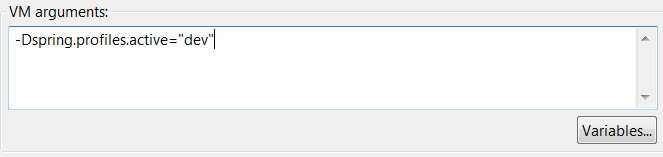
\includegraphics[width=0.8\textwidth]{Bilder/startlauncher.png}
    \caption{Profil über die VM-Arguments aktivieren}
    \label{fig:active-profile}
\end{figure}

\section{Konfiguration der Datenbank}\label{s_config_db}

\section{Konfiguration der Social-Login-Provider}\label{s_config_social}